\chapter{El problema inverso}%
\lhead{\thepage}
\rhead{\textit{El problema inverso}} \\
\vspace{0.01\textheight}
\label{sec:inverso}
%\pagebreak

En las secciones previas abordamos el problema directo de transporte 
de radiación en la materia mediante la ETR. En síntesis, el problema 
directo consta de, dados los parámetros ópticos $a(\x)$, $b(\x)$, la función  
de fase $\eta(\hth\cdot \hth')$, la velocidad de la luz en el medio participante 
$c$, las fuentes internas $s$ y las condiciones iniciales y de contorno, 
encontrar la solución $\ut$ a la ecuación~\eqref{eq:RTE}.

Para el problema inverso en tomografía óptica, alguno de los parámetros 
ópticos es desconocido, 
o conocido sólo parcialmente, y se dispone de mediciones experimentales 
de detectores colocados en el contorno del dominio que se quiere analizar. 
A partir de las mediciones experimentales de estos detectores, 
el objetivo es la reconstrucción de uno o más de los parámetros ópticos. 
En el caso de tomografía por fluorescencia y tomografía de bioluminiscencia, lo que se intenta reconstruir 
son las fuentes $s$ en la ec.~\eqref{eq:RTE}~\cite{Klose2005,Klose2009,Ren2010}, 
que vienen relacionadas a los coeficientes de absorción de los 
cromoforos y fluoroforos. 

En el contexto de esta tesis, nos limitaremos a la reconstrucción del 
coeficiente de absorción, $a(\x)$. La reconstrucción de dicho coeficiente 
encuentra aplicaciones en tomografía de fluorescencia, y en tomografía óptica. 
La reconstrucción de las propiedades de absorción en tomografía óptica 
 permite la identificación de tumores~\cite{Zhu2005,Zhu2010,Fujii2016b}, 
la obtención de imagenes funcionales del cerebro humano~\cite{Boas2001,bluestone2001,Arridge1999}, 
y la caracterización de diferentes constituyentes del tejido 
humano para la obtención de imágenes en medicina. En 
este trabajo nos enfocamos en la reconstrucción del coeficiente 
de absorción, pero los algorítmos y las estrategias propuestas 
pueden ser fácilmente generalizadas para la reconstrución 
de otros parámetros. 

Generalmente, para aplicaciones 
en diágnostico y monitoreo en el tratamiento de tumores, 
se asume cierta información previa 
para el coeficiente de dispersión, 
$b(\x)$, obtenida por técnicas de obtención 
de imagenes de alta resolución~\cite{Althobaiti2017,Guven2003} \eg Resonancia Magnética. 
Este conocimiento previo obtenido por otras técnicas, también brinda 
información límitada en el parámetro óptico de absorción $a(\x)$, 
como pueden ser los coeficientes de absorción para ciertos tejidos óseos, 
o el aire en regiones como la traquea del cuello humano, como también 
se conocen cotas superiores e inferiores para dicho parámetro, 
lo que permite restringir el espacio de funciones donde se busca minimizar 
la función objetivo. El uso de técnicas de alta resolución, como la Resonancia 
Magnética, posee ciertas límitaciones, como el alto costo, la baja disponibilidad 
de este tipo de aparatos 
(lo que impone una dificultad a la hora de seguir la evolución de un tratamiento 
asistido por diagnóstico de imágenes), y adicionalmente los dispositivos 
utilizados en tomografía óptica son portables, lo que permite tenerlos disponibles 
para su uso en diversas situaciones. En la figura~\ref{fig:esquemainv} esquematizamos los problemas directos e inverso, tal como son 
tratados en esta tésis. 


\begin{figure}[h!]
\centering
  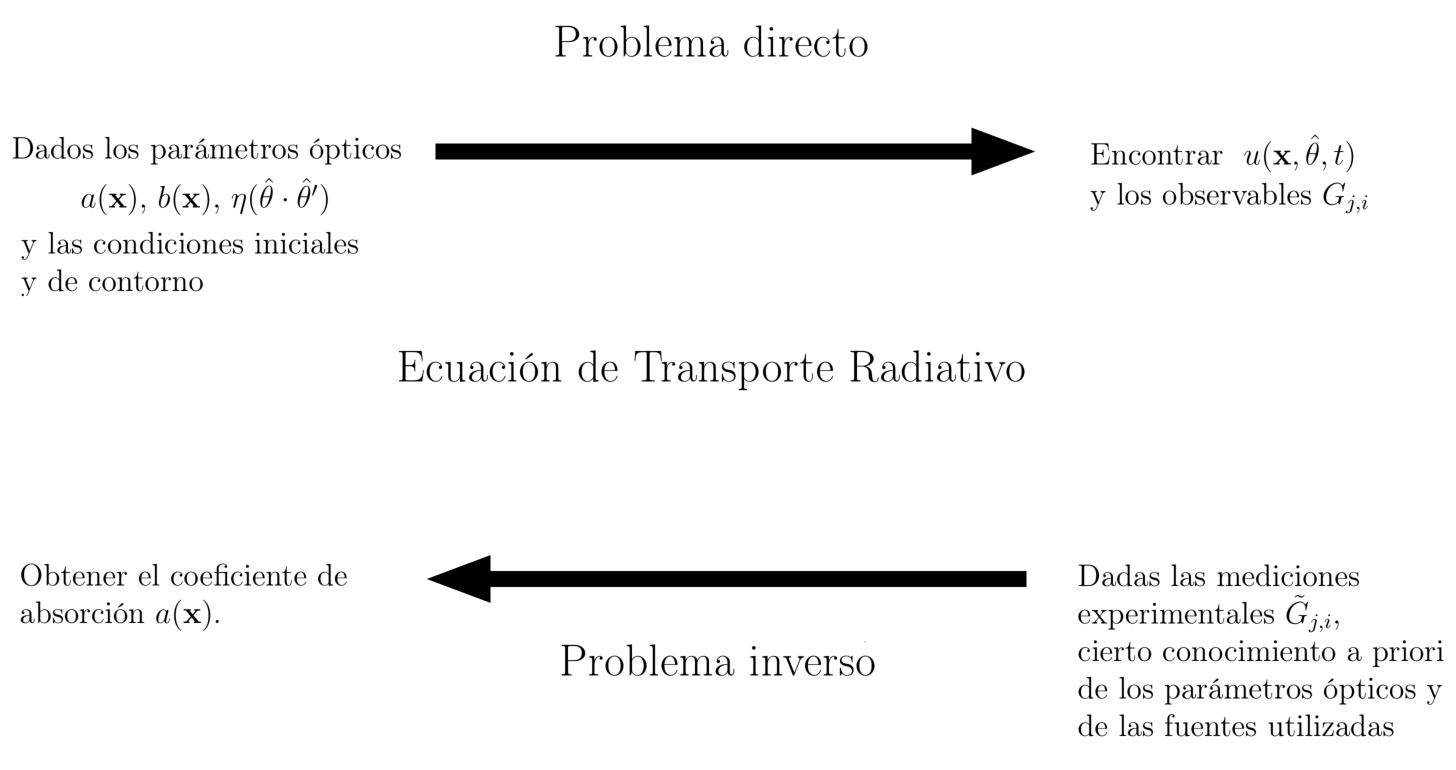
\includegraphics[width=\linewidth]{figuras/inv.pdf}\\
  \caption{
Grafico esquematico de los problemas directo e inverso, tal como son considerados 
en esta tésis.}
 \label{fig:esquemainv}
\end{figure}
Para la resolución del problema inverso, utilizamos el esquema \textit{MOBIR}, 
presentado en la sección siguiente. 

\section{El esquma \textit{MOBIR}}

\begin{wrapfigure}{l}{0.48\textwidth}
  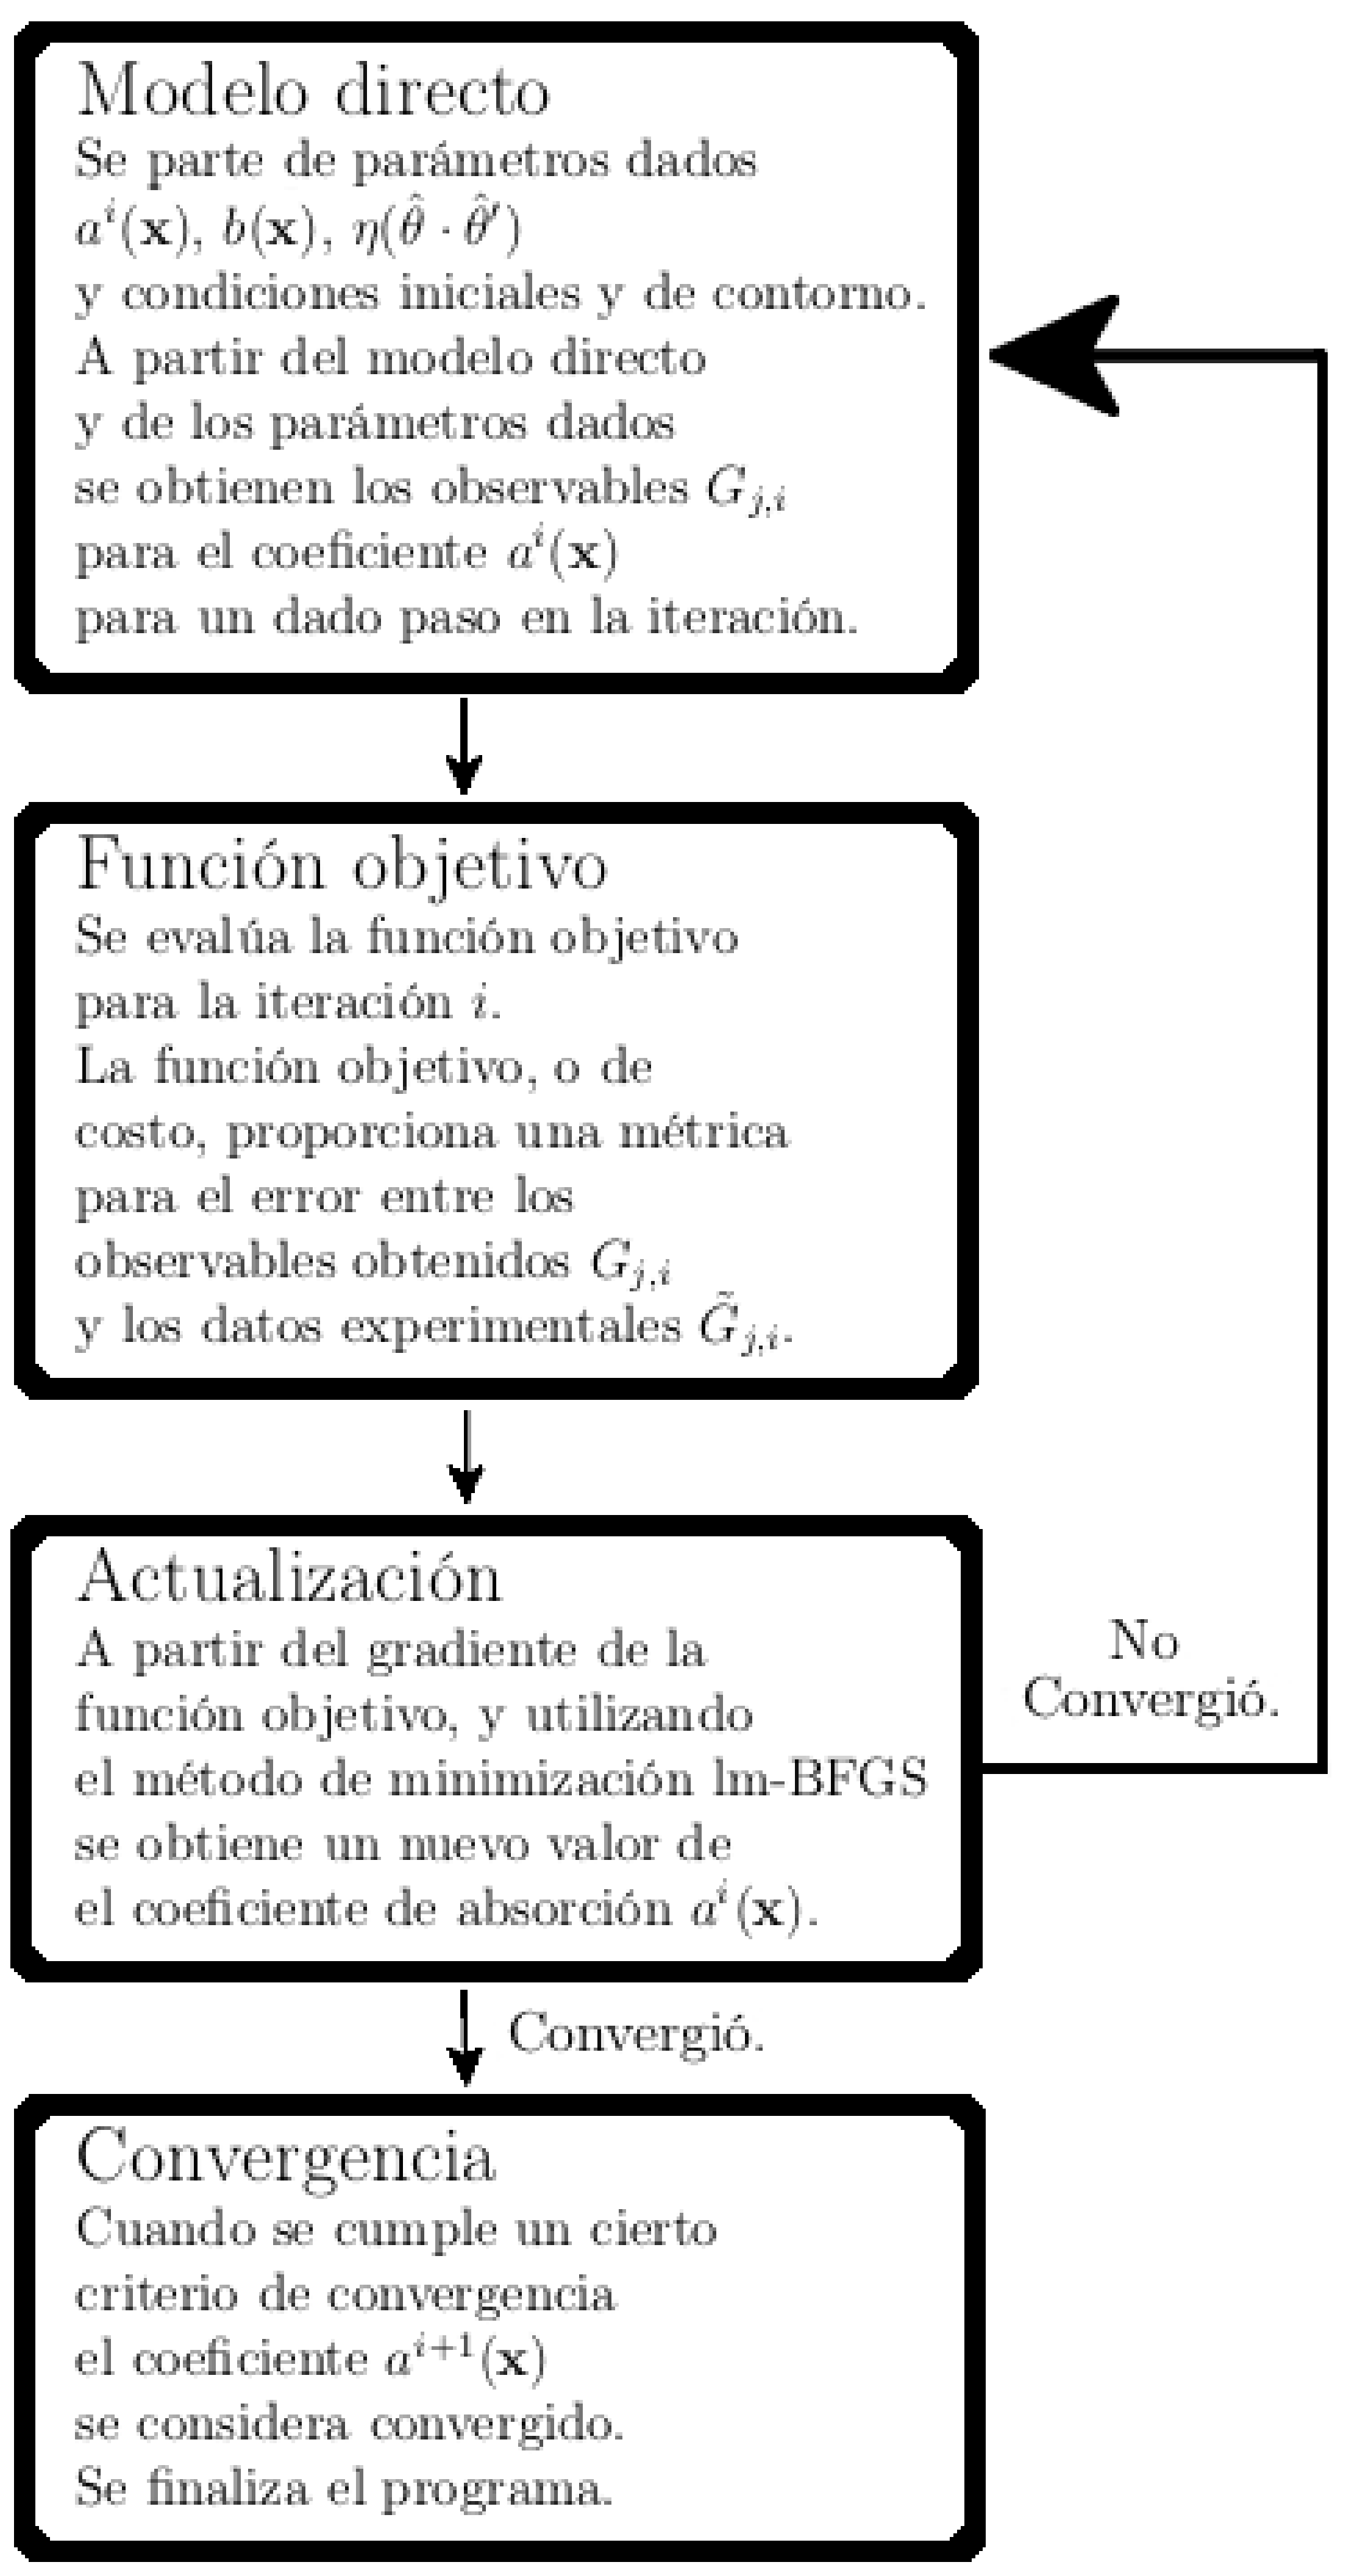
\includegraphics[width=0.48\textwidth]{figuras/mobir.eps}\\
  \caption{Esquema  MOBIR. El modelo directo es utilizado para obtener los observables simulados. Se evalúa el error entre los datos experimentales y los simulados por medio de la función objetivo. 
  Luego, utilizando un método de minimización, se actualiza el coeficiente $a(\x)^{i+1}$ a 
  ser utilizado en la iteración subsiguiente, hasta cumplir 
  un cierto criterio de convergencia. }
 \label{fig:mobir}
\end{wrapfigure}

En este tesis desarrollamos un algoritmo tipo MOBIR~\cite{Hielscher1999,Kim2010} (del inglés, {\em Model Based Iterative Image  
Reconstruction}). Este tipo de esquemas se basan en un modelo físico, y un método de minimización 
iterativo para la reconstrucción del parámetro deseado en el problema inverso.

El modelo físico utilizado es la Ecuación de Transporte Radiativo~\eqref{eq:RTE}. 
Para la minimización del funcional objetivo (que será introducido en una sección posterior) emplearemos el método de minimización 
de Broyden–Fletcher–Goldfarb–Shanno (BFGS) con uso de memoria reducido 
(lm-BFGS, de su sigla en inglés)~\cite{Byrd1995}. 

El problema inverso en tomografía óptica es resuelto como un problema de optimización 
no lineal. A partir de un valor inicial para el coeficiente de absorción $a(\x)^0$, 
el coeficiente de absorción es buscado de forma iterativa, actualizando su valor 
en cada iteración mediante el método lm-BFGS, el cual es un caso particular 
de los métodos de cuasi-Newton~\cite{Nocedal2006,Klose2003QN,Ren2006}. 
Partiendo del valor inicial $a(\x)^0$, el cual en general es estimado 
a partir de información obtenida de manera previa por otros métodos de imagenes, 
el coeficiente de absorción es 
\clearpage
\noindent actualizado en cada paso de la iteración $i+1$, según~\cite{Klose2003QN}
\begin{equation}
\mathbf{a}(\x)^{i+1}=\mathbf{a}(\x)^{i}+\alpha^i  \mathbf{d}^i(\x)
\label{eq:update}
\end{equation}
donde $\mathbf{a}(\x)^{i}$ debe ser interpretado como el 
vector obtenido a partir de el coeficiente de absorción en el 
dominio espacial $\Omega$  
discretizado, con $\alpha^i$ el largo del paso de Newton (que lo consideraremos 
en general $\alpha^i=1$), y $\mathbf{d}^i(\x)$ 
la dirección de descenso. En el caso del método de Newton (o {\em steepest descent}), la dirección de 
descenso vendrá dada por el gradiente $\mathbf{d}^i(\x)=-\nabla_a g(\x) $ de la función objetivo $g[u[\mathbf{a}]](\x)$ (que será definida posteriormente). 
En el contexto de esta tesis emplearemos el método lm-BFGS, ya que este método a 
mostrado ser eficiente en el contexto de tomografía óptica~\cite{Klose2003QN,Ren2006,
Prieto2017}. 

\section{El método de minimización BFGS}
Siguiendo a Nocedal~\cite{Nocedal2006}, el método BFGS parte de considerar la expansión de Taylor a segundo orden de la función objetivo 
que buscamos minimizar, la cual estará evaluada para el coeficiente $\mathbf{a}(\x)$,  
lo notaremos, por simplicidad  $g[\mathbf{a}]$

\begin{equation}
g[\mathbf{a}^i+ \mathbf{d}^i]\approx g[\mathbf{a}^i]+ (\mathbf{d}^i)^T \nabla_a g[\mathbf{a}^i]+\frac{1}{2}(\mathbf{d}^i)^T \nabla_a^2 g[\mathbf{a}^i+t\mathbf{d}^i] \mathbf{d}^i=m(\mathbf{d}^i).
\label{eq:Taylor}
\end{equation}
donde $t \in (0,1)$, y $(\mathbf{d}^i)^T$ indica el vector traspuesto a $\mathbf{d}^i$.
Además, si $g$ es al menos dos veces diferenciable se cumple qué 
\begin{equation}
\nabla_a g[\mathbf{a}^i+ \mathbf{d}^i]\approx \nabla_a g[\mathbf{a}^i]+\int_0^1\nabla_a^2 g[\mathbf{a}^i+t\mathbf{d}^i] \mathbf{d}^idt 
\label{eq:Taylor2}
\end{equation}
para algún $t \in (0,1)$.
Exigiendo que se anule la derivada de $m(\mathbf{d^i})$, se llega la dirección de Newton, dada por
\begin{equation}
\mathbf{d}^i=-(\nabla_a^2 g^i )^{-1} \nabla_a g^i.
\label{eq:direccion}
\end{equation}
El principal obstaculo para la aplicación de la dirección de Newton es la 
necesidad de calcular la inversa del Hessiano de la función objetivo, $\nabla_a^2 g^i$, 
lo cual en tomografía óptica, debido a la alta dimensionalidad de la ETR, puede 
resultar extremadamente costoso. 

Por este motivo, el método BFGS implementa una aproximación al Hessiano que 
es actualizada a cada paso de la iteración. Sumando y restando el término $ \nabla_a^2 g \mathbf{d}^i$ en la ecuación~\eqref{eq:Taylor2} se llega a
\begin{equation}
\nabla_a g[\mathbf{a}^i+ \mathbf{d}^i]\approx \nabla_a g[\mathbf{a}^i]+ \nabla_a^2 g[\mathbf{a}^i]\mathbf{d}^i + \int_0^1   \left( \nabla_a^2 g[\mathbf{a}^i+t\mathbf{d}^i]-\nabla_a^2 g[\mathbf{a}^i] \right)\mathbf{d}^idt
\label{eq:Taylor3}
\end{equation}
Dado que se asume la continuidad de $\nabla_a g$, el término de la integral 
es $o(||\mathbf{a}^{i+1}-\mathbf{a}^{i}||)$. Tomando $\mathbf{d}^i=\mathbf{a}^{i+1}-\mathbf{a}^{i}$ se llega a la relación
\begin{equation}
\begin{split}
\begin{aligned}
\nabla_a g[\mathbf{a}^{i+1}] &\approx \nabla_a g[\mathbf{a}^i]+ \nabla_a^2 g[\mathbf{a}^{i+1}-\mathbf{a}^i]  + o(||\mathbf{a}^{i+1}-\mathbf{a}^{i}||).\\
\therefore \nabla_a^2 g[\mathbf{a}^{i+1}-\mathbf{a}^i]& \approx \nabla_a g[\mathbf{a}^{i+1}]  - \nabla_a g[\mathbf{a}^{i}].
\end{aligned}
\end{split}
\label{eq:Taylor4}
\end{equation}
Esta última relación nos permite aproximar el Hessiano utilizando las derivadas de 
la función objetivo. 
El Hessiano es aproximado exigiendo que se cumpla la última relación en~\eqref{eq:Taylor4}
\begin{equation}
(B^{i+1})^{-1}y^i=s^i,
\label{eq:Taylor5}
\end{equation}
con $s_i=  \mathbf{a}^{i+1}-\mathbf{a}^{i}$ y $y^i=\nabla_a g[\mathbf{a}^{i+1}]  - \nabla_a g[\mathbf{a}^{i}]$. La fórmula BFGS para actualizar el Hessiano en cada iteración viene dada por~\cite{Nocedal2006}
\begin{equation}
(B^{i+1})^{-1}=(V^i)^T (B^{i})^{-1}V^i + \rho^i s^i (s^i)^T  ,
%B^{i}-\frac{B^{i}s^i (s^i)^T B^i }{(s^i)^TB^i s^i}+ \frac{y^i (y^i)^T}{(y^i)^T s^i}
\label{eq:HBFGS}
\end{equation}
la cual cumple la relación~\eqref{eq:Taylor5}, donde $\rho^i=\frac{1}{(y^i)^T s^i}$ 
y $V^i=\id - \rho^i y^i (s^i)^T$. 
La dirección de descenso, finalmente, se obtiene de la ecuación~\eqref{eq:direccion} reemplazando 
el Hessiano por su aproximación $B^i$
\begin{equation}
\mathbf{d}^{i}=-(B^{i})^{-1} \nabla_a g[\mathbf{a}^i]. 
\label{eq:HBFGS}
\end{equation}

\subsection{El método de uso de memoria limitada lm-BFGS}
En nuestro algoritmo para la resolución del problema inverso, el coeficiente 
de absorción es actualizado en cada iteración utilizando la relación 

\begin{equation}
\mathbf{a}(\x)^{i+1}=\mathbf{a}(\x)^{i}-(B^{i})^{-1} \nabla_a g[\mathbf{a}^i]
\label{eq:update2}
\end{equation}
Debido a que la aproximación a la inversa del Hessiano, $(B^i)^{-1}$, en tomografía óptica es una matriz 
que para el problema 2D discretizado, con $N_x \times N_y$ puntos 
en cada coordenada espacial tendrá dimensiones  $B^i\in \mathbb{R}^{N_x \times N_y}$, 
la manipulación y almacenamiento de esta matriz puede ser sumamente costosa. Por ello, 
para evitar la manipulación y el almacenamiento de esta matriz, se utiliza 
una versión aproximada de $(B^i)^{-1}$, para la cual se almacenan los vectores $\{s^k, y^k\}$, 
$k=i-m,...,i-1$ para un dado número de puntos $m$ previos a la iteración $i$-esima. 
Para esto se utiliza una aproximación inicial al Hessiano $(B^i)^{-1}_0$
\begin{equation}
(B^i)^{-1}_0=\gamma^i \id,\quad \quad \gamma^i=\frac{(s^{i-1})^T y^{i-1}}{(y^{i-1})^Ty^{i-1}},
\label{eq:initHess}
\end{equation}
y utilizando la ecuación~\eqref{eq:HBFGS} se tiene la relación de recurrencia
\begin{equation}
\begin{split}
\begin{aligned}
(B^{i+1})^{-1}=&(V^{i-1})^T...V^{i-m})^T) (B^i)^{-1}_0 (V^{i-m}...V^{i-1})  \\
&+\rho^{i-m} (V^{i-1})^T...V^{i-m+1})^T)s^{i-m} (s^{i-m})^T(V^{i-m+1}...V^{i-1+1}) \\
&+\rho^{i-m+1} (V^{i-1})^T...V^{i-m+2})^T)s^{i-m+1} (s^{i-m+1})^T(V^{i-m+2}...V^{i-1}) \\
&+...\\
&+\rho^{i-1} s^{i-1} (s^{i-1})^T. 
\end{aligned}
\end{split}
\label{eq:HBFGSrec}
\end{equation}
de donde se tiene el algoritmo~\eqref{algbfgs}~\cite{Byrd1995,Nocedal2006}

\begin{algorithm}
\caption{lm-BFGS}\label{algbfgs}
\begin{algorithmic}[1]
\State  $q = \nabla_a g[\mathbf{a}^i]$
\State \textbf{para} $k=i-1,i-2,\ldots,i-m$ hacer 
\State \hskip 0.75em $\alpha^k  = \rho^k (s^k)^T q$,
\State \hskip 0.75em $q  = q- \alpha^k y^k$,
\State \textbf{terminar}
\State $r = (B_0^k)^{-1} q$,
\State \textbf{para} $k=i-m,i-m+1,\ldots,i-1$ hacer 
\State \hskip 0.75em $\beta  = \rho^k (y^k)^T r$,
\State \hskip 0.75em $r  = r+s^k(\alpha^k-\beta)$,
\State \textbf{terminar}
\State Finalizar programa, con $(B^k)^{-1}\nabla_a g[\mathbf{a}^k]=r$.
\end{algorithmic}
\end{algorithm}  
  
En esta tesis utilizaremos el algoritmo lm-BFGS para encontrar 
el mínimo de la función objetivo. En todos los casos, usaremos el valor 
de $m=5$.
\section{El operador de transporte}

\section{Cálculo del gradiente de la función objetivo mediánte el formalismo 
del operador adjunto}
\section{Reconstrucciones numéricas}
\label{sec:inverseres}
\section{Consecuencias de la capa límite}
